\documentclass{standalone}
\usepackage{tikz}


\begin{document}

\begin{tikzpicture}
\linespread{1}


\coordinate (O) at (0,0,0);
\node at (O){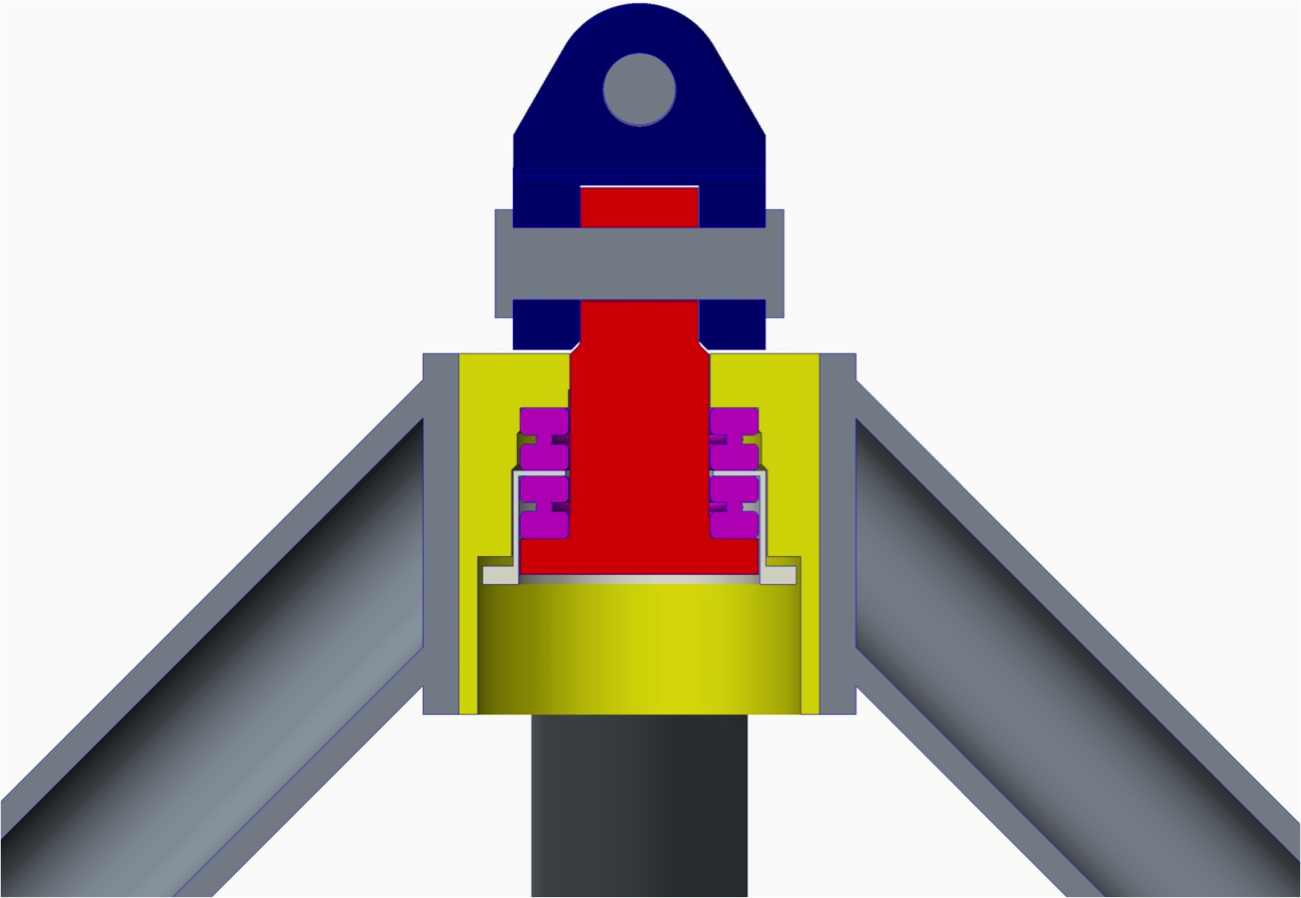
\includegraphics[width=0.8\textwidth]{Figures/rotator.png}};

\coordinate (bolts) at (3,3,0);
\node[right] at (bolts){Grade 8 bolts};

\draw (1,1.7,0) -- (bolts.west);
\draw (0,3.2,0) -- (bolts.west);

\draw (O) -- (-4,2.25,0)node[left]{Steel alloy pin};
\draw (-1,2.8,0) -- (-4,3,0)node[left]{Steel alloy pivot};
\draw (1.4,0,0) -- (3,2,0)node[right]{Titanium holder};

\draw (-1,0,0) -- (-4,1.5,0)node[left]{Steel ball bearing};
\draw (-1,-0.5,0) -- (-4,1,0)node[left]{Ceramic ball bearing};
\draw (-1.3,-1.2,0) -- (-4,0,0)node[left,align=right]{Attaches to\\ stepper shaft};
\draw (-1.6,-2,0) -- (-4,-1,0)node[left,align=right]{Attaches to\\ stepper body};


\end{tikzpicture}
\end{document} 